\subsection{Arquitectura del sistema}
\label{subsection:impl_propia}

	El presente trabajo, como se dijo con anterioridad, sienta sus bases en el trabajo realizado por Wang et al. salvo que el enfoque del mismo se centra en los problemas de reconocmiento de caracteres y el reconocimiento de palabras. En las próximas subsecciones, se procederá a explicar cuestiones de implementación que se tuvieron en cuenta al momento de resolver ambos problemas.

	\subsubsection{Reconocimiento de caracteres}

		\paragraph{Pipeline de procesamiento} ~\\

			La implementación que se realizó en este trabajo, está basada en un pipeline similar al que realizaron Wang et al. que abarca desde la construcción del dataset hasta la obtención de los resultados de clasificación. El pipeline se puede apreciar en la siguiente imagen.

	Construcción Dataset $\Rightarrow$(Extracción de Características $\Rightarrow$  Entrenamiento del Clasificador) $\Rightarrow$  Evaluación del clasificador

        \JS{por ahí se puede distinguir dos instancias del sistema: a tiempo de
        entrenamiento y a tiempo de test o de ejecución}


			\begin{figure}[htbp]
				\centering
				\fbox{ 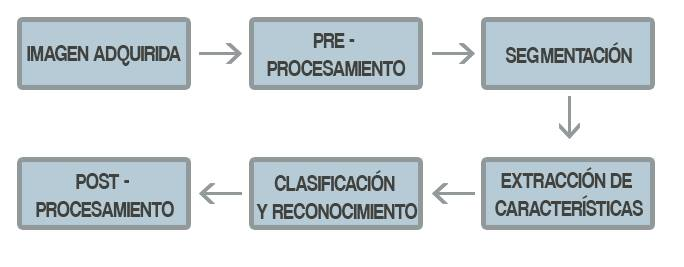
\includegraphics[scale=0.5]{img/OCR_pipeline_1.jpg} }
				\caption{Pipeline de procesamiento. Esto es un ejemplo de como quedaría visualmente pero no es el pipeline de este trabajo.}
				\label{fig: Pipeline de mi sistema}
			\end{figure}

		\paragraph{Generación de datos sintéticos} ~\\

                \JS{el dataset es uno solo. Lo que se hace generando muestas
                  sintéticas es agregar vistas de los caracteres que no están
                  reflejadas en el dataset original pero que son plausibles de
                  ser observadas en la realidad}
			Si bien el título hace referencia a un solo dataset , en el trabajo se hacen uso de múltiples datasets que evaluan diferentes puntos de vista del problema de reconocimiento. Lo que se intenta explicar aquí, es la creación general de los datasets, es decir, como se obtienen las imágenes sintéticas que conforman el dataset para que logren asemejarse a las imágenes reales.

			Inicialmente, se tiene como base un conjunto el cual contiene imágenes de caracteres de diversas fuentes. Lo que se busca, es aplicar a cada imagen un conjunto de transformaciones afines aleatorias con el objetivo final de obtener una imagen nueva con la apariencia de una real. Dichas transformaciones, toman a la imagen y le aplican de manera aleatoria cambios en la rotación, el tamaño, la inclinación, le aplican suavizado gaussiano (blur) y ruido, entre otras transformaciones. Un punto a destacar en este proceso, es que las fuentes de letras están en una escala de grises y se mantienen de esta forma. Esto es debido a que, durante el entrenamiento, solo es posible obtener las características de las imágenes sí y sólo sí estas están en escala de grises (requerimiento del algoritmo HOG). Otro tipo de transformación que vale la pena destacar, es la de anexar dos caracteres a los costados de la imagen a transformar. Esto es debido a que la mayoría de las imágenes de caracteres reales son extraidas de imágenes donde la misma forma parte de una palabra como cabría esperarse. Es por eso que en la mayoría de los datasets, cada caracter está acompañado de pedazos de otros caracteres.

			La creación de estos datasets son para el conjunto de entrenamiento del clasificador. El conjunto de test esta conformado por 15 imágenes reales por clase obtenidas del dataset \textit{Chars74K}, a las cuales no se les modifico en absoluto. Esto es debido a que los experimentos de evaluación del clasificador que se realizen tienen que poder ser comparados con los de Wang et al. en iguales condiciones.


		\paragraph{Entrenamiento del clasificador}  ~\\

			La segunda etapa del pipeline corresponde al entrenamiento del clasificador. Al igual que los autores del trabajo original, en este se utiliza como clasificador a Random Ferns. Para poder entrenar al clasificador, se procede a extraer las características de las imágenes del dataset a través del algoritmo HOG. HOG devuelve en sí un vector $v \in \mathbb{R}^{n}$ (donde $n$ depende de los parámetros que se le pasen al algoritmo, explicado en el próximo capítulo) el cual hay que binarizar para poder almacenarlo.

			Para poder binarizar los vectores calculados, como se explicó en la sección \ref{subsection:hog}, se necesita de un umbral cuya dimensión es igual a la de los vectores. Dicho umbral binariza a un vector comparando sus valores dimensión a dimensión. Un vez realizado este procedimiento, los vectores modificados se almacenan en un diccionario. Este último, esta estructurado como un conjunto de diccionarios anidados y representa la base ``base de datos'' del sistema. Los detalles del porqué se eligió esta forma de almacenar la información se puede encontrar en el apéndice A. \RC{Crear apendice A donde se van a discutir cosas como lenguaje usado, base de datos, librerias entre otros}

			Dado que los vectores pertenecen al conjunto $\{ 0,1 \}^{N}$ si los quisiéramos almacenar en una sola tabla (habría una tabla por clase), cada una debería tener $2^{N}$ entradas lo cual si $N$ es muy grande sería imposible por la cantidad de memoria necesitada para mantener estas tablas en memoria. Luego, basándonos en lo explicado sobre Random Fern en \cite{subsection:ferns}, la solución pasa por dividir cada vector en $M$ grupos de dimensión $S = \frac{N}{M}$. Con esto, un vector completo esta almacenado en $M$ tablas diferentes (tablas correspondiente a la clase del vector). En total estaríamos trabajando con $M \times 62$ tablas (pues hay 62 clases diferentes).

			Dado un vector $v=(v_1, \dots, v_s)$ donde $v_i \in \{ 0,1 \}^{M}$, $z$ sea la clase de $v$ y sean $t_i i=1, \dots, s$ las tablas de $z$. Cada grupo $v_i i=1, \dots, s$ va a tener una entrada en su tabla correspondiente $z_i$ equivalente a su representación decimal. Inicialmente cada tabla está inicializada dado un parámetro $\alpha \neq 0$ que se explicará en detalle en el próximo capítulo.

		\paragraph{Evaluación del clasificador} ~\\

			Para la evaluación del clasificador, se toma como conjunto de test el descripto en la sección de creación del dataset. A cada imágen del conjunto de test, se le extrae el descriptor HOG, se lo binariza y con el vector resultante se calcula la probabilidad de que dicho vector perteneza a cada una de las clases involucradas. El calculo para cada clase es el mismo y consiste en dividir el vector de prueba en $M$ grupos y por cada grupo obtener el valor en la tabla correspondiente. Por cada clase entonces tendríamos $M$ valores. Finalmente se realiza la suma de los logaritmos de cada valor y el resultado es la probabilidad de que ese vector pertenzca a la clase evaluada. Como es claro, al final se le asigna a la imagen evaluada la clase que haya obtenido la mayor probabilidad.

	\subsubsection{Reconocimiento de palabras}

		\RC{Todavía no he implementado nada de esto así que queda pendiente...}